\begin{tikzpicture}
	\node[anchor = south east,inner sep=0pt] at (0,10) {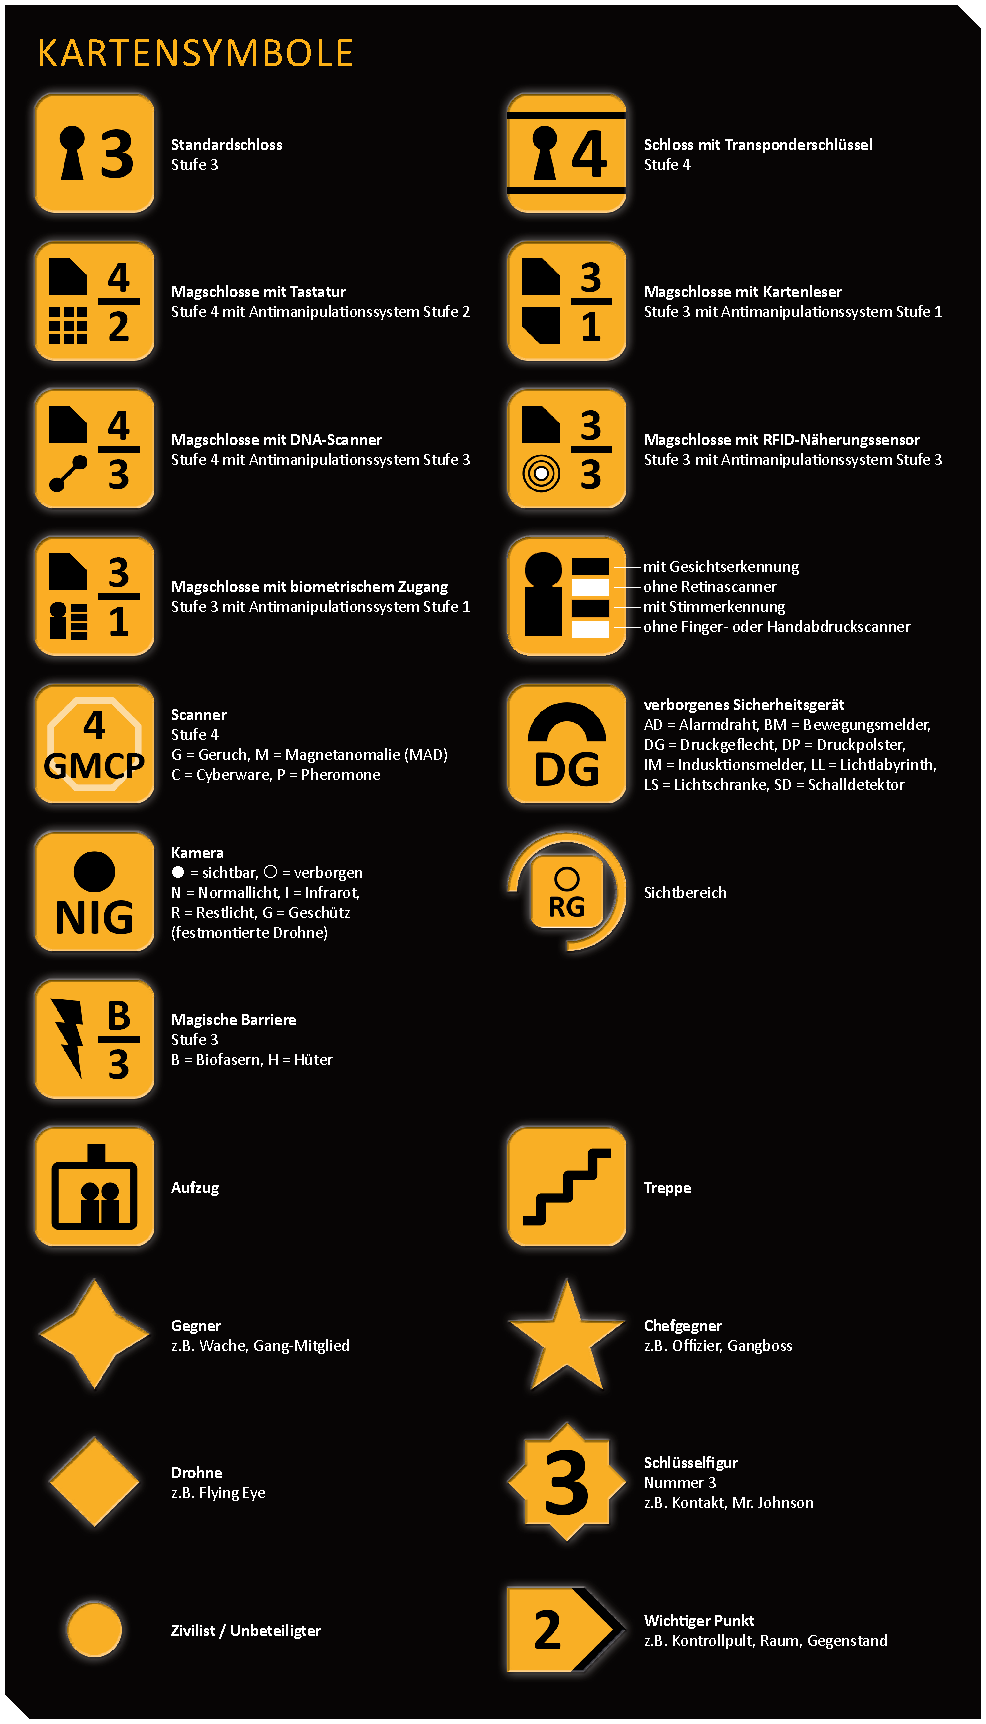
\includegraphics[height =10cm]{graphics/Legende}};
	\draw[white] (0,0) -- (20,0) -- (20,20) -- (0,20) -- (0,0);
	\node[inner sep=0pt] at (-3,9.5) {10 Meter};
	\draw[thick] (-5,9) -- (-1,9);
	\draw[thick] (-5,9.25) -- (-5,8.75);
	\draw[thick] (-1,9.25) -- (-1,8.75);
	\draw[thick] (1,19) -- (17,19) -- (17,5) -- (19,5) -- (19,1) -- (5,1) -- (5,5) -- (6,5) -- (6,11) -- (1,11) -- (1,19);
	\draw[thick] (5,2) -- (6,2) -- (6,5);
	\draw[thick] (7,1) -- (7,4);
%	\draw[thick] (8,1) -- (8,4);	
%	\draw[thick] (10,1) -- (10,4);
	\draw[thick] (11,1) -- (11,4);
%	\draw[thick] (13,1) -- (13,4);
	\draw[thick] (15,1) -- (15,4);
	\draw[thick] (6,5) -- (17,5);
	\draw[thick] (6,5) -- (17,5);
	\draw[thick] (7,4) -- (17,4) -- (17,1);
	\draw[thick] (19,2) -- (18,2) -- (18,5);
%	\draw[thick] (6,11) -- (6,14.5) -- (1,14.5);
	\draw[thick] (6,11) -- (6,19);
%	\draw[thick] (6,19) -- (6,16) -- (1,16);
	
	
	\draw[thick,lightgray] (17,17.25) -- (1,17.25);
	\draw[thick,lightgray] (17,17.25-3.5) -- (1,17.25-3.5);
	\draw[thick,lightgray] (17,17.25-7) -- (6,17.25-7);
	\draw[thick,lightgray] (17,17.25-10.5) -- (6,17.25-10.5);
	\draw[thick,lightgray] (12.5,19) -- (12.5,5);
	\draw[thick,lightgray] (7.5,19) -- (7.5,5);
	
	
%	\foreach \i in {1,...,4}{
%	\draw[thick, fill=brown] (\i+7,19) rectangle (\i+8,18);
%	\draw[thick, fill=brown] (\i+12,19) rectangle (\i+13,18);
%	
%	
%	\draw[thick, fill=brown] (\i+7,15.5) rectangle (\i+8,16.5);
%	\draw[thick, fill=brown] (\i+12,15.5) rectangle (\i+13,16.5);
%	\draw[thick, fill=brown] (\i+7,14.5) rectangle (\i+8,15.5);
%	\draw[thick, fill=brown] (\i+12,14.5) rectangle (\i+13,15.5);
%	
%	\draw[thick, fill=brown] (\i+7,13) rectangle (\i+8,12.0);
%	\draw[thick, fill=brown] (\i+12,13) rectangle (\i+13,12);
%	\draw[thick, fill=brown] (\i+7,11.0) rectangle (\i+8,12.0);
%	\draw[thick, fill=brown] (\i+12,11) rectangle (\i+13,12);
%	
%	\draw[thick, fill=brown] (\i+7,13-3.5) rectangle (\i+8,12-3.5);
%	\draw[thick, fill=brown] (\i+12,13-3.5) rectangle (\i+13,12-3.5);
%	\draw[thick, fill=brown] (\i+7,11.0-3.5) rectangle (\i+8,12.0-3.5);
%	\draw[thick, fill=brown] (\i+12,11-3.5) rectangle (\i+13,12-3.5);
%	
%	\draw[thick, fill=brown,] (6,13-7) rectangle (7,12-7);
%		\draw[thick, fill=brown,] (\i+6,13-7) rectangle (\i+7,12-7);
%		\draw[thick, fill=brown,] (\i+12,13-7) rectangle (\i+13,12-7);
%    }
	
%	\draw[gray,thick]  (5.75,1) -- (5.25,1) -- (5.25,0.5) arc (90:180:-0.5);
	\draw[gray,thick]  (6,4.25) -- (6,4.75) -- (6.5,4.75) arc (-180:-270:-0.5);
	\draw[gray,thick]  (18,4.25) -- (18,4.75) -- (17.5,4.75) arc (180:270:0.5);
%	\draw[gray,thick]  (18.75,1) -- (18.25,1) -- (18.25,0.5) arc (90:180:-0.5);
%	\draw[gray,thick]  (17.75,5) -- (17.25,5) -- (17.25,5.5) arc (-90:-180:-0.5);
%	\draw[gray,thick]  (7.75,4) -- (7.25,4) -- (7.25,3.5) arc (90:180:-0.5);
%	\draw[gray,thick]  (9.75,4) -- (9.25,4) -- (9.25,3.5) arc (90:180:-0.5);
	\draw[gray,thick]  (10.75,4) -- (10.25,4) -- (10.25,3.5) arc (90:180:-0.5);
%	\draw[gray,thick]  (12.75,4) -- (12.25,4) -- (12.25,3.5) arc (90:180:-0.5);
	\draw[gray,thick]  (13.75,4) -- (13.25,4) -- (13.25,3.5) arc (90:180:-0.5);
	\draw[gray,thick]  (15.75,4) -- (15.25,4) -- (15.25,3.5) arc (90:180:-0.5);
		
%	\draw[gray,thick]  (11.75,5) -- (11.25,5) -- (11.25,4.5) arc (90:180:-0.5);
%	\draw[gray,thick]  (11.75,5) -- (12.25,5) -- (12.25,4.5) arc (-90:-180:0.5);
%	\draw[gray,thick]  (2.75,14.5) -- (2.25,14.5) -- (2.25,14) arc (90:180:-0.5);
%	\draw[gray,thick]  (2.75,14.5) -- (3.25,14.5) -- (3.25,14) arc (-90:-180:0.5);
	
	\draw[gray,thick]  (6,17.25) -- (6,17.75) -- (5.5,17.75) arc (0:90:-0.5);
	\draw[gray,thick]  (6,17.25) -- (6,16.75) -- (5.5,16.75) arc (-0:-90:-0.5);
	
	\draw[gray,thick]  (6,17.25-3.5) -- (6,17.75-3.5) -- (5.5,17.75-3.5) arc (0:90:-0.5);
	\draw[gray,thick]  (6,17.25-3.5) -- (6,16.75-3.5) -- (5.5,16.75-3.5) arc (-0:-90:-0.5);
	
%	\draw[gray,thick]  (17,17.25) -- (17,17.75) -- (16.5,17.75) arc (0:90:-0.5);
%	\draw[gray,thick]  (17,17.25) -- (17,16.75) -- (16.5,16.75) arc (-0:-90:-0.5);
%	\draw[gray,thick]  (17,13.25+0.5) -- (17,13.75+0.5) -- (16.5,13.75+0.5) arc (0:90:-0.5);
%	\draw[gray,thick]  (17,13.25+0.5) -- (17,12.75+0.5) -- (16.5,12.75+0.5) arc (-0:-90:-0.5);
%	\draw[gray,thick]  (17,9.25+1) -- (17,9.75+1) -- (16.5,9.75+1) arc (0:90:-0.5);
%	\draw[gray,thick]  (17,9.25+1) -- (17,8.75+1) -- (16.5,8.75+1) arc (-0:-90:-0.5);
%	\draw[gray,thick]  (17,9.25-2.5) -- (17,9.75-2.5) -- (16.5,9.75-2.5) arc (0:90:-0.5);
%	\draw[gray,thick]  (17,9.25-2.5) -- (17,8.75-2.5) -- (16.5,8.75-2.5) arc (-0:-90:-0.5);
	
%	\draw[gray,thick]  (2.75,16) -- (2.25,16) -- (2.25,16.5) arc (270:180:-0.5);
%	\draw[gray,thick]  (2.75,16) -- (3.25,16) -- (3.25,16.5) arc (-270:-180:0.5);
	

	
	\Level[Treppenhaus,0.05] at (5.5,4);
	\Level[Treppenhaus,0.05] at (18.5,4);
	
%	\MLBio[5,4,GR,0.05] at (16,4);
	\magBarr[Hueter,4, 0.05] at (16,2.5);
	\magBarr[Hueter,4, 0.05] at (13,2.5);
	\magBarr[Hueter,4, 0.05] at (9,2.5);

%	
%	\NSC[drohne, 0.05] at (6.5,17.25);
%	\NSC[drohne, 0.05] at (6.5,17.25-3.5);
%	\NSC[drohne, 0.05] at (2.5,17.25);
%	\NSC[drohne, 0.05] at (2.5,17.25-3.5);
%	\NSC[drohne, 0.05] at (4.5,17.25);
%	\NSC[drohne, 0.05] at (4.5,17.25-3.5);
%	\NSC[drohne, 0.05] at (6.5,17.25-7);
%	\NSC[drohne, 0.05] at (6.5,17.25-10.5);
%	\NSC[drohne, 0.05] at (7.5,18.5);
%	\NSC[drohne, 0.05] at (12.5,18.5);
%	
%
%	
%	\cam[verborgen,NR,0900-1200,0.05] at (6.75,1.25);
%	\cam[verborgen,NR,0300-0600,0.05] at (6.25,4.75);
%	\cam[verborgen,NR,0600-0900,0.05] at (17.75,4.75);
%	\cam[verborgen,NR,1200-0300,0.05] at (17.25,1.25);
%	


\end{tikzpicture}